\title {
        \textbf{Pikachu's Revenge: Design Document} \\
}
\author {
Rebecca Hachey \\
Timothy Luciani \\
\textit{reh59@pitt.edu, tbl8@cs.pitt.edu}
}
\date {\today}

\documentclass[11pt,twocolumn]{article}

\newcommand{\tab}{\hspace*{3em}}

\usepackage{lingmacros}
\usepackage{tree-dvips}
\usepackage{graphicx}
\usepackage{fixltx2e}
\usepackage{verbatim}
\usepackage{amsmath}
\usepackage{framed}
\usepackage{algorithm}
\usepackage{algpseudocode} \usepackage{qtree}

\usepackage{tikz}
\usetikzlibrary{snakes}
\usepackage{fullpage}
\usepackage{varwidth}

\usepackage{mdframed}

\usepackage[paper=letterpaper,dvips,top=0.25in,left=0.25in,right=0.2in,
    foot=0.25in,bottom=0.25in]{geometry}

\setlength{\parindent}{0in}

\makeatletter
\renewcommand{\ALG@beginalgorithmic}{\tiny}
\makeatother

\begin{document}

 \maketitle

\section{Introduction} 

This design document presents the underlying features behind \textit{Pikachu's Revenge}'s \textit{myPTM}: my Pitt Transaction Manager. The goal of this system is to provide transactional limited support for a small database system by developing a concurrency control module, \textit{myPTM}. This control module will provide standard uncontrolled access to files while also providing both serialization and atomic access to the database using \textit{Strict Two-Phase Locking}. Our design aborts transactions due to deadlock while avoiding livelock all together by implementing the \textit{Wait for Graph} detection scheme. The following section outlines the overall design of the system.

\section{Design}

\begin{figure}[ht!]
\centering
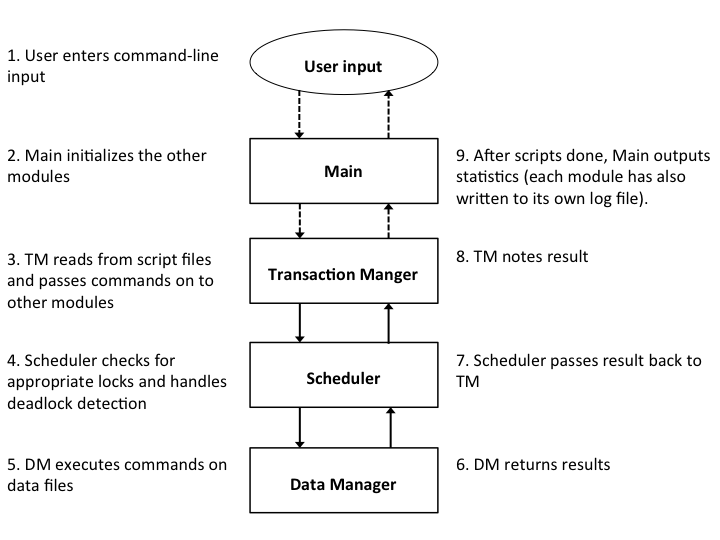
\includegraphics[width=100mm]{overalldesign.png}
\caption{The overall workflow of \textit{myPTM} as it executes commands from the user. }
\label{overflow}
\end{figure}

This section describes the implementation of \textit{myPTM}, including the data structures, variables, and functions to be implemented within each module. Figure 1. shows the workflow of our system. 

\subsection{Main / Entry Point}

This module serves as the main entry point of the transaction manager. The purpose of this module is to process requests from the user, executing the appropriate modules depending on the request. This module is also responsible for keeping track of the global data structures:

\begin{itemize}
 \item \textbf{transManager} --
 \item \textbf{scheduler} -- 
 \item  \textbf{dataManager} --
 \end{itemize}

each one corresponding to the module of the same name. The definition of \textit{myPTM}:\\

\noindent\fbox{%
\parbox{\textwidth}{
\begin{varwidth}{\dimexpr\linewidth-2\fboxsep-2\fboxrule\relax}
\begin{center}
\begin{algorithmic}[H]

    \State \textbf{Inputs}: (Command Line)
    \State \tab{list of script files}
    \State \tab{bufferSize}
     \State \tab{seed = random number generator}
     \State \tab{numBufferPages}
     \State \tab{readMode (0 = round robin, 1 = random}
      \State \tab{searchMode (0 = scan, 1 = hash)}
      \State {}
      \State \textbf{Outputs}: (console)
       \State \tab{numCommitted = \# of committed transactions}
        \State \tab{percentRead = \% of read operations}
         \State \tab{percentWrite = \% of write operations}
    	 \State \tab{avgResponseTime = average response time}
	\State \# Input and Output above
	\Function{main()} {} 
	\State main entry
	\EndFunction  
\end{algorithmic} 
\end{center} 
\end{varwidth} % 
} }  \\ \\


Studying the input and output above, the main module: takes in from the user the scripts; sets the buffer size and the number of buffer pages; initiates the random number see; and decides both the read mode and search mode. After execution of \textit{myPTM} is complete, the module outputs the number of committed transactions, the percent of both read and write operations, as well as the average response time of the entire execution, to the console or a log file for further analysis.

\subsection{ Transaction Manager }

The transaction manager in our system can be thought of as the main module of the system; driving execution of the commands executed by the user. After receiving the scripts from the main entry point, our transaction manager will read and parse the commands contained within each file concurrently and pass the new commands to the scheduler. To study effects our \textit{myPTM} in different scenarios of command execution time combinations, the transaction manager will either parse the files in a round robin or random fashion. 

Looking into more detail of this module, the transaction manager will have two data structures: 

\begin{itemize}
\item \textbf{currTrans} --list of currently executing transactions/processes and script files (TID - thread ID?, script filename) tuples
\item \textbf{transactionLog} --  tracks effects of currently running transactions.
\end{itemize}

This module will also have two variables that help drive the execution:

\begin{itemize}
\item \textbf{readMode} -- 0 (round robin) or 1 (random)
\item \textbf{logFile} --  - file handle for Transaction Manager log file
\end{itemize}

With the above definitions in mind, the transactions module will look like:\\

\noindent\fbox{%
\parbox{\textwidth}{
\begin{varwidth}{\dimexpr\linewidth-2\fboxsep-2\fboxrule\relax}
\begin{center}
\begin{algorithmic}[H]
    \Function{handleCommand}{command,TID,dataItem}
    \If{abort \&\& transaction}
    \State \textbf{undoEffects}(TID)
    \EndIf
   \State pass on to Scheduler
   \State after returned status/values
   \State update transactionLog
   \EndFunction
   \State
   \Function{undoEffects}{TID}
   \State  \# Undo effects of transaction with TID
   \EndFunction
   \State
    \State  \# Parse next commands to pass on to Scheduler
   \Function{parseCommands}{scriptFile, numCommands} 
    \State \For{$i = 1 \to numCommands$}
    \State extract next command from scriptFile
    \State \textbf{handleCommand}(command,TID,dataItem)
    \EndFor
    \EndFunction
\end{algorithmic} 
\end{center}
\end{varwidth} % 
}}

\subsection{Scheduler}

The scheduler of \textit{myPTM} implements \textit{Strict Two-Phase Locking (S2PL)} as its lock manager. This sub manager works as follows:

\begin{algorithmic}

	\If{T wants to read/write on an object}
	\State Obtains S/X lock.
	\State Holds lock until end of transaction 
	\EndIf
   
\end{algorithmic}  . \\

This locking scheme thus guarantees serializability, a recoverable schedule, avoidance of cascading aborts, and that the precedence graph will be acyclic. $myPTM$ employs the following data structure to handle the locking:

\begin{itemize}
\item \textbf{lockTable} - hash of lock entries: OID, Mode, List, List Wait queue
\subitem Number of transactions currently holding a lock
\subitem Type of lock held (shared or exclusive)
\subitem Pointer to queue of lock requests
\end{itemize}

The second submodule that the schedule controls is the deadlock detector. For this detection, \textit{myPTM} employs the \textit{Wait for Graph} deadlock detection scheme, where nodes of the graph are the transactions with edges from $node_i$ to $node_j$ represent a conflict of $node_i$ waiting for $node_j$. This submodule uses the data structure:

\begin{itemize}
\item \textbf{wfgMatrix} - keep track of dependencies 
\subitem TID
\subitem waitForTID
\end{itemize}

to keep track of the dependencies across the transactions. 

The following is how the module will be implemented. The variable \textbf{logFile} handles the scheduler's log: \\

\noindent\fbox{%
\parbox{\textwidth}{
\begin{varwidth}{\dimexpr\linewidth-2\fboxsep-2\fboxrule\relax}
\begin{center}
\begin{algorithmic}[H]
\State \# Ensures strict 2PL and then passes command on to Data Manager
\State \#Return value passed back by Data Manager or blocked status 
\Function {handleCommand}{command, TID, dataItem} 
\State type = use command to determine which lock needed
\If{read/multiple read/write/delete}
	\If{checkLock(type,TID, dataItem)}
		\State pass on to Data Manager
	\Else
		\State lockStatus = reqLock(type, TID,dataItem)
		\If{lockStatus == failure}
			\State add to lockTable, wfgMatrix
			\Return blocked
		\Else
			\State pass on to Data Manager
		\EndIf
	\EndIf	
	
\ElsIf{commit or abort}
	\State pass on to Data Manager
	\State \textbf{releaseLocks(TID)}
\Else
	\State error, unknown command
\EndIf

\EndFunction
	
\State \# Release locks TID has acquired:
\State \# Approve a pending request
\State \# Update lockTable, wfgMatrix
\Function{releaseLocks}{TID}  \EndFunction
\State \# Return true if TID has lock of type on dataItem; otherwise, return false
\Function{checkLock}{type, TID, dataItem} \EndFunction
\State \# Attempt to acquire lock of type on dataItem; return true on success, else false
\Function {reqLock}{type, TID, dataItem} \EndFunction

\end{algorithmic} 
\end{center}
\end{varwidth} % 
}}


\subsection{Data Manager}

The Data Manager maintains the data in the files and executes the actual reads and writes on the data files. It will receive commands through the Scheduler and pass the results of executing these commands back. The Data Manager will allow for different searching methods -- scan or hash. \\

The data structures will be:

\begin{itemize}
\item \textbf{writeBuffer} -- keeps track of uncommitted modifications to files
\item \textbf{dbFiles} -- list of data files
\end{itemize}

This module will also have the following variables:
\begin{itemize}
\item \textbf{searchMode} -- 0 (scan) or 1 (hash)
\item \textbf{bufferSize} -- number of buffer pages specified on command line for searching
\item \textbf{logFile} -- file handle for Data Manager log file
\end{itemize}

The following functions will be included in this module:\\

\begin{algorithmic}
	\State  \# Retrieve the record with id in filename
	\Function{read}{filename, id}
		\If{filename doesn't exist}
			\Return -2
		\EndIf
		\State  Search for record with id
		\If{record doesn't exist}
			\Return -1
		\EndIf	
	\EndFunction
	\State
	\State \# Retrieve the record(s) with areaCode in filename
	\Function{multRead}{filename, areaCode}
		\If{filename doesn't exist}
			\Return -2
		\EndIf
		\State  search for record(s) with areaCode
		\If{no such records exist}
			\Return -1
		\EndIf	
	\EndFunction
	\State
	\State \# Write the record into filename
	\Function{write}{filename, record}
		\If{filename doesn't exist}
			create file
		\EndIf
		\State write record
	\EndFunction
	\State
	\State \# Delete the filename
	\Function{delete}{filename}
	\EndFunction

\end{algorithmic} .\\

\section{Implementation}

We will implement myPTM in C++ on a Unix-based operating system. Within a file, records are stored in slotted pages whose size is 512 bytes. We will use fixed-length records, which will simplify access and reduce storage of administrative information for fields. 

\end{document}